\subsection{Why exocentric vision ?}
\frame
{
  \frametitle{Why exocentric vision ?}
  
  \textit{it's difficult for an operator not accustomed to the vehicle
    to estimate the vehicle's position and direction and the distances to a target strictly
    based on camera images from the first person viewpoint\footnote{\tiny{as stated by M. Sugimoto and others}}.}
  \pause
  
  \vskip15pt

  \alert{\texttt{Idea}}: an exocentric camera would provide a view of the robot in the operating
  environment and, thus, a better understanding of where the robot is located into the
  environment and its actual direction. \\
  
  \pause
    
  \vskip5pt
  
  \alert{\texttt{Trouble}}: exocentric camera could be mounted on a rear-mounted protuberance of the robot,
  but such a protuberance would terribly limit the robot activity and its moving abilities.
  
}

\frame
{
  \frametitle{Why exocentric vision ?}

  \alert{\texttt{Solution}}: simulate a virtual \textbf{exocentric} point of view, by drawing with augmented reality
  the robot on previous recorded first-person (i.e. \textbf{egocentric}) images, shot along its path. \\
  
  \vskip8pt
  \pause
  Fixed a previous image, actual robot is drawn in order to
  simulate what a \textbf{rear} camera would shoot.
  
  \vskip8pt
  \pause
  
  \begin{columns}
    
    \column{0.4\textwidth}
    \visible<3-> {
      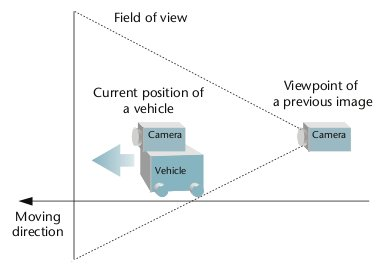
\includegraphics[width=\textwidth]{img/exocentric_vision.jpg}
    }

    \pause
    
    \column{0.2\textwidth}
    \visible<4-> {
      \begin{center}
        $\Longrightarrow$ \\
        \alert{virtual exocentric} (augmented reality)
      \end{center}
    }

    \pause

    \column{0.4\textwidth}
    \visible<5-> {
      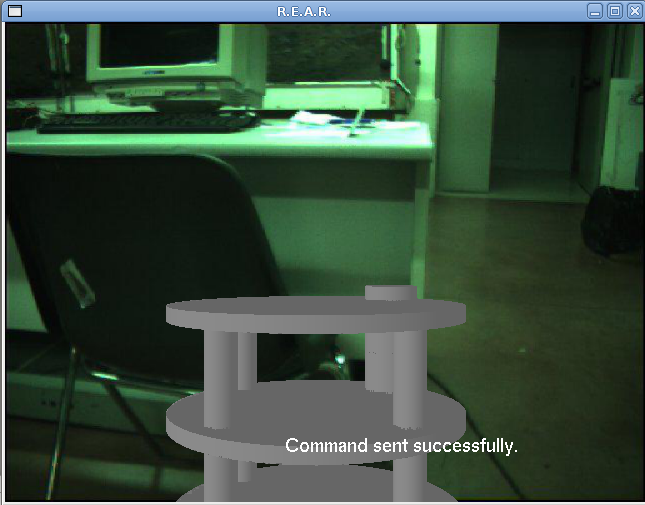
\includegraphics[width=\textwidth]{img/virtual_exocentric.jpg}
    }
    
  \end{columns}



}
